\begin{figure*}
\begin{tikzpicture}
[ plain/.style={ draw=none, fill=none, }, remember picture, net/.style={ matrix of nodes, nodes={ draw, circle,
    inner sep=7.5pt
    },
  nodes in empty cells,
  column sep=-10.5pt,
  row sep=0.8cm
  }
]
%\draw[help lines] (-3cm,-6cm) grid (6cm,3cm);
\matrix[net] (mat)
{
              & |[plain]| &           & |[plain]|  &           & |[plain]| &           &  |[plain]|      &               \\
    |[plain]| &           & |[plain]| &            & |[plain]| &           & |[plain]| &                 & |[plain]|     \\ 
    |[plain]| & |[plain]| &           & |[plain]|  &           & |[plain]| & 	  	   &  |[plain]|      & |[plain]|     \\ 
  };

  \node at ($(mat-1-1.west)+(-16pt,0)$) {Input: };
  \node at ($(mat-2-2.west)+(-24pt,0)$) {Hidden:};
  \node at ($(mat-3-2.west)+(-24pt,0)$) {Output:};
  \node at (mat-1-1.base) {$i_1$};
  \node at (mat-1-3.base) {$i_2$};
  \node at (mat-1-5.base) {...};
  \node at (mat-1-7.base) {$i_{n-1}$};
  \node at (mat-1-9.base) {$i_{n}$};
  \node at (mat-2-2.base) {$h_1$};
  \node at (mat-2-4.base) {$h_2$};
  \node at (mat-2-6.base) {$...$};
  \node at (mat-2-8.base) {$h_{m}$};
  \node at (mat-3-5.base) {$...$};

 \foreach \a in {1,3}{
    \foreach \b in {2,6}{
        \draw[->] (mat-1-\a.south) -- (mat-2-\b.north);
     }
  }
 \foreach \a in {3,7,9}{
    \foreach \b in {4,8}{
        \draw[->] (mat-1-\a.south) -- (mat-2-\b.north);
     }
  }

 \foreach \c in {2,4,6,8}{
    \foreach \d in {3,5,7}{
 		\draw[->] (mat-2-\c.south) -- (mat-3-\d.north);
	}
 }
\end{tikzpicture}
\caption{Neural Network Model}
\end{figure*}



\begin{figure}
\centering
\begin{tikzpicture}
    %\draw[help lines] (-3cm,-6cm) grid (6cm, 6cm);
    \tikzstyle{block} = [rectangle, text centered, draw=black,
    minimum width=1.1cm, minimum height=0.4cm]
    % first level
    \node (evaluation-parent) [block, minimum width=2.4cm, minimum
        height=1.8cm,draw=white] {};
    \node (evaluation) [block] at ($(evaluation-parent.north)$) {evaluation};
    \node (reproduction) [block] at ($(evaluation-parent.south)$) {reproduction};
    \node (tasks) [block, minimum width=1.1cm, minimum height=0.4cm] {tasks};

    \draw[->] ($(evaluation.south)+(0.3cm,0cm)$) --
        ($(tasks.north)+(0.3cm,0cm)$) node[auto=left, pos=0.5] {\small weights}; 
    \draw[<-] ($(evaluation.south)+(-0.3cm,0cm)$) --
        ($(tasks.north)+(-0.3cm,0cm)$) node[auto=right, pos=0.5] {\small fitness}; 

    % get intersection
    \draw[white] (evaluation.west) coordinate (A) -- ++(-1.5cm,0) coordinate (B);
    \draw[white] (reproduction.west) -- ++(-0.3cm,0) coordinate (C) -- ++(0,4cm) coordinate
        (D);
    \draw[black] (reproduction.west) -- ++(-0.3cm,0) -- (intersection cs:
        first line={(A)--(B)}, second line={(C)--(D)}) coordinate (E);
    \draw[->] (E) -- (evaluation.west);

    \draw[white] (evaluation.east) coordinate (E) -- ++(2cm,0) coordinate (F);
    \draw[white] (reproduction.east) -- ++(0.3cm,0) coordinate (G) -- ++(0,4cm) coordinate
        (H);
    \draw[<-] (reproduction.east) -- ++(0.3cm,0) -- (intersection cs:
        first line={(E)--(F)}, second line={(G)--(H)}) coordinate (I);
    \draw (I) -- (evaluation.east);

    % second level
    \node (level2) [block,draw=black, minimum width=3.5cm, minimum height=3.0cm] at
        (0cm,0.2cm) {};
    \node [align=left] at ($(level2.north)+(0,-0.2cm)$) {\tiny THE EVOLUTION
        OF};
    \node [align=left] at ($(level2.north)+(0,-0.45cm)$) {\tiny CONNECTION
            WEIGHTS 
        };
    % third level
    \node (level3-assister) [block, draw=white, minimum width=5cm, minimum
		height=4.6cm] at
        (0, 0.3cm)  {};
    \node (evaluation) [block] at ($(level3-assister.north)$) {\small evaluation of
        learning rules};
    \node (reproduction) [block] at ($(level3-assister.south)$) {\small reproduction of
        learning rules};

    \draw[->] ($(evaluation.south)+(0.3cm,0cm)$) --
        ($(level2.north)+(0.3cm,0cm)$) node[auto=left, pos=0.5] {\small learning
        rule}; 
    \draw[<-] ($(evaluation.south)+(-0.3cm,0cm)$) --
        ($(level2.north)+(-0.3cm,0cm)$) node[auto=right, pos=0.5] {\small fitness}; 

    \draw[white] (evaluation.west) coordinate (A) -- ++(-1.3cm,0) coordinate (B);
    \draw[white] (reproduction.west) -- ++(-0.3cm,0) coordinate (C) -- ++(0,4cm) coordinate
        (D);
    \draw[black] (reproduction.west) -- ++(-0.3cm,0) -- (intersection cs:
        first line={(A)--(B)}, second line={(C)--(D)}) coordinate (E);
    \draw[->] (E) -- (evaluation.west);

    \draw[white] (evaluation.east) coordinate (E) -- ++(2cm,0) coordinate (F);
    \draw[white] (reproduction.east) -- ++(0.3cm,0) coordinate (G) -- ++(0,4cm) coordinate
        (H);
    \draw[<-] (reproduction.east) -- ++(0.3cm,0) -- (intersection cs:
        first line={(E)--(F)}, second line={(G)--(H)}) coordinate (I);
    \draw (I) -- (evaluation.east);
   % fourth level
    \node (level4) [block, draw=black, minimum width=5.5cm, minimum
        height=6.0cm] at
        (0, 0.4cm)  {};
    \node [align=left] at ($(level4.north)+(0,-0.25cm)$) {\tiny THE EVOLUTION
        OF LEARNING RULES};
    % level five
    \node (level5-assister) [block, draw=white, minimum width=6.4cm, minimum
        height=7.0cm] at
        (0, 0.4cm)  {};
    \node (evaluation) [block] at ($(level5-assister.north)$) {\small evaluation of
        architecture};
    \node (reproduction) [block] at ($(level5-assister.south)$) {\small reproduction of
        learning architecture};

    \draw[white] (evaluation.west) coordinate (A) -- ++(-1.5cm,0) coordinate (B);
    \draw[white] (reproduction.west) -- ++(-0.6cm,0) coordinate (C) -- ++(0,4cm) coordinate
        (D);
    \draw[black] (reproduction.west) -- ++(-0.6cm,0) -- (intersection cs:
        first line={(A)--(B)}, second line={(C)--(D)}) coordinate (E);
    \draw[->] (E) -- (evaluation.west);

    \draw[white] (evaluation.east) coordinate (E) -- ++(2cm,0) coordinate (F);
    \draw[white] (reproduction.east) -- ++(0.6cm,0) coordinate (G) -- ++(0,4cm) coordinate
        (H);
    \draw[<-] (reproduction.east) -- ++(0.6cm,0) -- (intersection cs:
        first line={(E)--(F)}, second line={(G)--(H)}) coordinate (I);
    \draw (I) -- (evaluation.east);
    % level 6
    \node (level6) [block, minimum width=7.0cm, minimum
        height=8.1cm] at
        (0, 0.5cm)  {};
    \node [align=left] at ($(level6.north)+(0,-0.2cm)$) {\tiny THE EVOLUTION OF
            ARCHITECTURE
        };
\end{tikzpicture}
\caption{Genetic algorithm and artificial neural network}
\end{figure}


In this paper, the feedforward nueural network models are adopted in our
system, because feedforward NNs are straigntforward and simply to code.  For
funnction approximation, Cybenko demonstrated that a two-lay multilayer
perceptron(MLP) is capbable of forming an arbitrarily close approximation to
any continusous nonliner mapping\cite{cybenko1989approximation}. Therefore, the
we propose a GNN framework as shown in Figure \ref{fig:gnn}. The search space
is parametrized by: (i) the number of nodes m(possibly unbounded) in hidden
layer, to narrow down the search space, m is less than n; (ii) the type of
operation every nodes executes, e.g., sigmoid, linear, gaussian. (iii) the
connection relationship between hidden nodes and inputs.


\begin{figure}[ht]
	\centering
	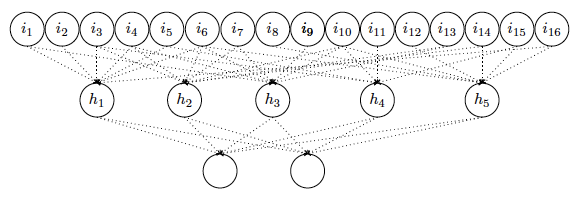
\includegraphics{./a0_figure_ann_for_clt_architecture_example1.tex}
	\label{fig:parent1}
	\caption{bbbbbbb}
\end{figure}



%%\begin{figure}
%\centering
\begin{tikzpicture}
	[ p/.style={ draw=none, fill=none, }, remember picture, 
	  net/.style={ matrix of nodes, nodes={ draw, circle, inner sep=7.5pt },
	  nodes in empty cells,
	  column sep=-10.5pt,
	  row sep=0.8cm
	  }
	]
%\draw[help lines] (-3cm,-6cm) grid (6cm,3cm);
\matrix[net] (mat)
{
		  & |[p]| &  & |[p]| &  & |[p]| &  & |[p]| &  & |[p]| &  & |[p]| &  & |[p]| &  & |[p]| &  &
			|[p]| &  & |[p]| &  & |[p]| &  & |[p]| &  & |[p]| &  & |[p]| &  & |[p]| &  & |[p]|    \\
	 |[p]| & |[p]| & |[p]| &  |[p]| &        & |[p]| & |[p]| & |[p]| &|[p]| &       & |[p]| &  |[p]| & |[p]| &
	 |[p]| &       & |[p]| &  |[p]| &  |[p]| & |[p]| & |[p]| &       &|[p]| & |[p]| & |[p]| & |[p]|
		   & |[p]| &       &  |[p]| &  |[p]| & |[p]| & |[p]| & |[p]| &|[p]| \\ 
	 |[p]| &  |[p]| & |[p]|  &  |[p]| & |[p]|  &  |[p]| &  |[p]| &  |[p]| & |[p]| & |[p]| & |[p]| &       & |[p]|
		   &  |[p]| & |[p]|  &  |[p]| &        &  |[p]| &  |[p]| &  |[p]| & |[p]| & |[p]| & |[p]| & |[p]| &     |[p]|
		   &  |[p]| & |[p]|  &  |[p]| & |[p]|  &  |[p]| &  |[p]| &  |[p]| \\ 
	  };
	  \node at (mat-1-1.base)  {$i_1$};
	  \node at (mat-1-3.base)  {$i_2$};
	  \node at (mat-1-5.base)  {$i_3$};
	  \node at (mat-1-7.base)  {$i_4$};
	  \node at (mat-1-9.base)  {$i_5$};
	  \node at (mat-1-11.base)  {$i_6$};
	  \node at (mat-1-13.base)  {$i_7$};
	  \node at (mat-1-15.base)  {$i_8$};
	  \node at (mat-1-17.base)  {$i_9$};
	  \node at (mat-1-17.base)  {$i_9$};
	  \node at (mat-1-19.base)  {$i_{10}$};
	  \node at (mat-1-21.base)  {$i_{11}$};
	  \node at (mat-1-23.base)  {$i_{12}$};
	  \node at (mat-1-25.base)  {$i_{13}$};
	  \node at (mat-1-27.base)  {$i_{14}$};
	  \node at (mat-1-29.base)  {$i_{15}$};
	  \node at (mat-1-31.base)  {$i_{16}$};

	  \node at (mat-2-5.base)  {$h_1$};
	  \node at (mat-2-10.base) {$h_2$};
	  \node at (mat-2-15.base) {$h_3$};
	  \node at (mat-2-21.base) {$h_4$};
	  \node at (mat-2-27.base) {$h_5$};
		 \foreach \a in {1,3,5,7,9,11,31}{
				\draw[->,dotted] (mat-1-\a.south) -- (mat-2-5.north);
			 }
		 \foreach \a in {5,7,11,13,19,25,27}{
				\draw[->,dotted] (mat-1-\a.south) -- (mat-2-10.north);
			 }
		 \foreach \a in {1,7,11,13,17,19,25}{
				\draw[->,dotted] (mat-1-\a.south) -- (mat-2-15.north);
			 }
		 \foreach \a in {5,9,19,21,29}{
				\draw[->,dotted] (mat-1-\a.south) -- (mat-2-21.north);
			 }
		 \foreach \a in {11,15,19,23,27,29,31}{
				\draw[->,dotted] (mat-1-\a.south) -- (mat-2-27.north);
			 }
		 \foreach \c in {5,10,15,21,27}{
			\foreach \d in {12,17}{
				\draw[->,dotted] (mat-2-\c.south) -- (mat-3-\d.north);
			}
 }
\end{tikzpicture}
%\caption{Parent 1\label{fig:parents1}}
%\end{figure}

\begin{figure*}
\centering
\begin{tikzpicture}
[ p/.style={ draw=none, fill=none, }, remember picture, 
  net/.style={ matrix of nodes, nodes={ draw, circle, inner sep=7.5pt },
  nodes in empty cells,
  column sep=-10.5pt,
  row sep=0.8cm
  }
]
%\draw[help lines] (-3cm,-6cm) grid (6cm,3cm);
\matrix[net] (mat)
{
	  & |[p]| &  & |[p]| &  & |[p]| &  & |[p]| &  & |[p]| &  & |[p]| &  & |[p]| &  & |[p]| &  &
	    |[p]| &  & |[p]| &  & |[p]| &  & |[p]| &  & |[p]| &  & |[p]| &  & |[p]| &  & |[p]|    \\
 |[p]| &  |[p]|& |[p]| &        &  |[p]| &       & |[p]| &       &|[p]| &       & |[p]| &   & |[p]| &
       &  |[p]|&       &  |[p]| &       & |[p]| &       &|[p]| &       & |[p]| &  
	   & |[p]| &       &  |[p]| &  |[p]| & |[p]| & |[p]| & |[p]| &|[p]| & |[p]| \\ 
 |[p]| &  |[p]| & |[p]|  &  |[p]| & |[p]|  &  |[p]| &  |[p]| &  |[p]| & |[p]| & |[p]| & |[p]| &       & |[p]|
	   &  |[p]| & |[p]|  &  |[p]| &        &  |[p]| &  |[p]| &  |[p]| & |[p]| & |[p]| & |[p]| & |[p]| &     |[p]|
	   &  |[p]| & |[p]|  &  |[p]| & |[p]|  &  |[p]| &  |[p]| &  |[p]| \\ 
  };
  \node at (mat-1-1.base)  {$i_1$};
  \node at (mat-1-3.base)  {$i_2$};
  \node at (mat-1-5.base)  {$i_3$};
  \node at (mat-1-7.base)  {$i_4$};
  \node at (mat-1-9.base)  {$i_5$};
  \node at (mat-1-11.base)  {$i_6$};
  \node at (mat-1-13.base)  {$i_7$};
  \node at (mat-1-15.base)  {$i_8$};
  \node at (mat-1-17.base)  {$i_9$};
  \node at (mat-1-17.base)  {$i_9$};
  \node at (mat-1-19.base)  {$i_{10}$};
  \node at (mat-1-21.base)  {$i_{11}$};
  \node at (mat-1-23.base)  {$i_{12}$};
  \node at (mat-1-25.base)  {$i_{13}$};
  \node at (mat-1-27.base)  {$i_{14}$};
  \node at (mat-1-29.base)  {$i_{15}$};
  \node at (mat-1-31.base)  {$i_{16}$};

  \node at (mat-2-5.base)  {$h_1$};
  \node at (mat-2-10.base) {$h_2$};
  \node at (mat-2-15.base) {$h_3$};
  \node at (mat-2-21.base) {$h_4$};
  \node at (mat-2-27.base) {$h_5$};
 \foreach \a in {13,15,17,19,21}{
        \draw[->] (mat-1-\a.south) -- (mat-2-4.north);
     }
 \foreach \a in {1,3,5,7}{
        \draw[->] (mat-1-\a.south) -- (mat-2-6.north);
     }
 \foreach \a in {1,3,5,7,17,19,21,23}{
        \draw[->] (mat-1-\a.south) -- (mat-2-8.north);
     }
 \foreach \a in {5,9,11,13,15}{
        \draw[->] (mat-1-\a.south) -- (mat-2-10.north);
     }
 \foreach \a in {23,27,29,31}{
        \draw[->] (mat-1-\a.south) -- (mat-2-12.north);
     }
 \foreach \a in {11,15,19}{
        \draw[->] (mat-1-\a.south) -- (mat-2-14.north);
     }
 \foreach \a in {27,29,31}{
        \draw[->] (mat-1-\a.south) -- (mat-2-16.north);
     }
 \foreach \a in {11,19,27,31}{
        \draw[->] (mat-1-\a.south) -- (mat-2-18.north);
     }
 \foreach \a in {15,19,23}{
        \draw[->] (mat-1-\a.south) -- (mat-2-20.north);
     }
 \foreach \a in {3,5,7}{
        \draw[->] (mat-1-\a.south) -- (mat-2-22.north);
     }
 \foreach \a in {17,19,21,23}{
        \draw[->] (mat-1-\a.south) -- (mat-2-24.north);
     }
 \foreach \a in {21,23,25,27,29}{
        \draw[->] (mat-1-\a.south) -- (mat-2-26.north);
     }
 \foreach \c in {4,6,8,10,12,14,16,18,20,22,24,26}{
    \foreach \d in {12,17}{
 		\draw[->] (mat-2-\c.south) -- (mat-3-\d.north);
	}
 }

\end{tikzpicture}
\caption{Neural Network Model}
\end{figure*}


\begin{table}[h!]
	\centering
		\caption{first table}
		\begin{tabular}{l|cccc cccc cccc cccc}
			\toprule
hi    & $i_1$ & $i_2$ & $i_3$ & $i_4$ & $i_5$ & $i_6$ & $i_7$ & $i_8$ & $i_9$ & $i_{10}$ & $i_{11}$ & $i_{12}$ & $i_{13}$ & $i_{14}$ & $i_{15}$ & $i_{16}$ \\
			\midrule
$h_1$ & 1  & 1 & 1  & 1  & 1 & 1 & 0 & 0  & 0 & 0 & 0 & 0  & 0 & 0  & 1 & 1 \\
$h_2$ & 0  & 1 & 1  & 1  & 0 & 0 & 0 & 1  & 0 & 0 & 1 & 1  & 0 & 0  & 0 & 0 \\
$h_3$ & 1  & 0 & 0  & 1  & 0 & 1 & 1 & 0  & 1 & 1 & 0 & 0  & 1 & 0  & 0 & 0 \\
$h_4$ & 0  & 0 & 1  & 0  & 1 & 0 & 0 & 0  & 0 & 1 & 0 & 1  & 0 & 0  & 1 & 0 \\
$h_5$ & 0  & 0 & 0  & 0  & 0 & 1 & 0 & 1  & 0 & 1 & 0 & 1  & 0 & 1  & 1 & 1 \\
			\bottomrule
		\end{tabular}
\end{table}


\begin{figure*}
\centering
\begin{tikzpicture}
[ p/.style={ draw=none, fill=none, }, remember picture, 
  net/.style={ matrix of nodes, nodes={ draw, circle, inner sep=7.5pt },
  nodes in empty cells,
  column sep=-10.5pt,
  row sep=0.8cm
  }
]
%\draw[help lines] (-3cm,-6cm) grid (6cm,3cm);
\matrix[net] (mat)
{
	  & |[p]| &  & |[p]| &  & |[p]| &  & |[p]| &  & |[p]| &  & |[p]| &  & |[p]| &  & |[p]| &  &
	    |[p]| &  & |[p]| &  & |[p]| &  & |[p]| &  & |[p]| &  & |[p]| &  & |[p]| &  & |[p]|    \\
 |[p]| & |[p]| & |[p]|   & |[p]|  &  |[p]| &  |[p]| & |[p]| &|[p]|  &   & |[p]| &      & |[p]| &  &  |[p]| &  &
 |[p]| &       & |[p]| &   & |[p]|   &  & |[p]| &       &|[p]| & |[p]| & |[p]| & |[p]|
	   & |[p]| &  |[p]|   &  |[p]| &  |[p]| & |[p]| & |[p]|  \\ 
 |[p]| &  |[p]| & |[p]|  &  |[p]| & |[p]|  &  |[p]| &  |[p]| &  |[p]| & |[p]| & |[p]| & |[p]| &       & |[p]|
	   &  |[p]| & |[p]|  &  |[p]| &        &  |[p]| &  |[p]| &  |[p]| & |[p]| & |[p]| & |[p]| & |[p]| &     |[p]|
	   &  |[p]| & |[p]|  &  |[p]| & |[p]|  &  |[p]| &  |[p]| &  |[p]| \\ 
  };
  \node at (mat-1-1.base)   {$i_1$};    \node at (mat-1-3.base)   {$i_2$}; 
  \node at (mat-1-5.base)   {$i_3$};    \node at (mat-1-7.base)   {$i_4$}; 
  \node at (mat-1-9.base)   {$i_5$};    \node at (mat-1-11.base)  {$i_6$}; 
  \node at (mat-1-13.base)  {$i_7$};    \node at (mat-1-15.base)  {$i_8$}; 
  \node at (mat-1-17.base)  {$i_9$};    \node at (mat-1-17.base)  {$i_9$};
  \node at (mat-1-19.base)  {$i_{10}$}; \node at (mat-1-21.base)  {$i_{11}$};
  \node at (mat-1-23.base)  {$i_{12}$}; \node at (mat-1-25.base)  {$i_{13}$};
  \node at (mat-1-27.base)  {$i_{14}$}; \node at (mat-1-29.base)  {$i_{15}$};
  \node at (mat-1-31.base)  {$i_{16}$};

  \node at (mat-2-9.base)  {$h_1$};
  \node at (mat-2-11.base) {$h_2$};
  \node at (mat-2-13.base) {$h_3$};
  \node at (mat-2-15.base) {$h_4$};
  \node at (mat-2-17.base) {$h_5$};
  \node at (mat-2-19.base) {$h_6$};
  \node at (mat-2-21.base) {$h_7$};
  \node at (mat-2-23.base) {$h_8$};

 \foreach \a in {1,3,5,7,9,11,31}{
        \draw[->,dotted] (mat-1-\a.south) -- (mat-2-9.north);
     }
 \foreach \a in {5,7,11,13,19,25,27}{
        \draw[->,dotted] (mat-1-\a.south) -- (mat-2-11.north);
     }
 \foreach \a in {27,29,31}{
        \draw[->,dashed] (mat-1-\a.south) -- (mat-2-13.north);
     }
 \foreach \a in {11,19,27,31}{
        \draw[->,dashed] (mat-1-\a.south) -- (mat-2-15.north);
     }
 \foreach \a in {15,19,23}{
        \draw[->,dashed] (mat-1-\a.south) -- (mat-2-17.north);
     }
 \foreach \a in {3,5,7}{
        \draw[->,dashed] (mat-1-\a.south) -- (mat-2-19.north);
     }
 \foreach \a in {17,19,21,23}{
        \draw[->,dashed] (mat-1-\a.south) -- (mat-2-21.north);
     }
 \foreach \a in {21,23,25,27,29}{
        \draw[->,dashed] (mat-1-\a.south) -- (mat-2-23.north);
     }

 \foreach \c in {9,11,13,15,17,19,21,23}{
    \foreach \d in {12,17}{
 		\draw[->] (mat-2-\c.south) -- (mat-3-\d.north);
	}
 }

\end{tikzpicture}
\caption{Child}
\end{figure*}






\begin{figure}[h!]
\centering
	\resizebox{.7\linewidth}{!}{
\begin{tikzpicture}
    %\draw[help lines] (-3cm,-6cm) grid (6cm, 6cm);
    \tikzstyle{block} = [rectangle, text centered, draw=black,
    minimum width=1.1cm, minimum height=0.4cm]
	% first level evolution: connection weights
    \node (evaluation-parent) [block, minimum width=2.4cm, minimum
        height=1.8cm,draw=white] {};
    \node (evaluation) [block] at ($(evaluation-parent.north)$) {evaluation};
    \node (reproduction) [block] at ($(evaluation-parent.south)$) {reproduction};
    \node (tasks) [block, minimum width=1.1cm, minimum height=0.4cm] {tasks};

    \draw[->] ($(evaluation.south)+(0.3cm,0cm)$) --
        ($(tasks.north)+(0.3cm,0cm)$) node[auto=left, pos=0.5] {\small weights}; 
    \draw[<-] ($(evaluation.south)+(-0.3cm,0cm)$) --
        ($(tasks.north)+(-0.3cm,0cm)$) node[auto=right, pos=0.5] {\small fitness}; 

	\draw[black] (reproduction.west) -- ++(-0.3cm,0)  |- (evaluation.west);
	\draw[black] (reproduction.east) -- ++(0.3cm,0)   |- (evaluation.east);

    \node (level1) [block,draw=black, minimum width=3.5cm, minimum height=3.0cm] at
        (0cm,0.2cm) {};
    \node [align=left] at ($(level1.north)+(0,-0.2cm)$) {\tiny THE EVOLUTION
        OF};
    \node [align=left] at ($(level1.north)+(0,-0.45cm)$) {\tiny CONNECTION
            WEIGHTS
        };
    % second level evolution: active functions
    \node (level2_container) [block, draw=black, minimum width=5.8cm, minimum
        height=6.0cm] at
        (0, 0.4cm)  {};
    \node [align=left] at ($(level2_container.north)+(0,-0.25cm)$) {\tiny THE EVOLUTION
        OF ACTIVE FUNCTIONS};
    \node (level2-assister) [block, draw=white, minimum width=5cm, minimum
		height=4.6cm] at
        (0, 0.3cm)  {};
    \node (evaluation) [block] at ($(level2-assister.north)$) {\small evaluation of
        active functions};
    \node (reproduction) [block] at ($(level2-assister.south)$) {\small reproduction of
        active functions};

    \draw[->] ($(evaluation.south)+(0.3cm,0cm)$) --
        ($(level1.north)+(0.3cm,0cm)$) node[auto=left, pos=0.5] {\small active functions
        }; 

    \draw[<-] ($(evaluation.south)+(-0.3cm,0cm)$) --
        ($(level1.north)+(-0.3cm,0cm)$) node[auto=right, pos=0.5] {\small fitness}; 

	\draw[black] (reproduction.west) -- ++(-0.3cm,0)  |- (evaluation.west);
	\draw[black] (reproduction.east) -- ++(0.3cm,0)   |- (evaluation.east);
    % third level: evolution of learning rules
    \node (level3-assister) [block, draw=white, minimum width=3cm, minimum
        height=7.6cm] at
        (0, 0.4cm)  {};
	\node (level3_container) [block, draw=black, minimum width=7.5cm, minimum
		height=9cm] at (0, 0.4cm)  {};
    \node [align=left] at ($(level3_container.north)+(0,-0.25cm)$) {\tiny THE EVOLUTION
        OF LEARNING RULES};
    \node (evaluation) [block] at   ($(level3-assister.north)$) {\small evaluation of
        learning rules};
    \node (reproduction) [block] at ($(level3-assister.south)$) {\small reproduction of
        learning rules};
    \draw[->] ($(evaluation.south)+(0.3cm,0cm)$) --
        ($(level2_container.north)+(0.3cm,0cm)$) node[auto=left, pos=0.5] {\small learning
        rule}; 
    \draw[<-] ($(evaluation.south)+(-0.3cm,0cm)$) --
        ($(level2_container.north)+(-0.3cm,0cm)$) node[auto=right, pos=0.5] {\small fitness}; 

	\draw[black] (reproduction.west) -- ++(-0.9cm,0)  |- (evaluation.west);
	\draw[black] (reproduction.east) -- ++(0.9cm,0)   |- (evaluation.east);

	% fourth level: evolution of topology
    \node (level4-assister) [block, draw=white, minimum width=3cm, minimum
        height=11cm] at
        (0, 0.8cm)  {};
	\node (level4_container) [block, draw=black, minimum width=9cm, minimum
		height=11.8cm] at (0, 0.8cm)  {};
    \node (evaluation) [block] at   ($(level4-assister.north)$) {\small evaluation of
        topology};
    \node (reproduction) [block] at ($(level4-assister.south)$) {\small reproduction of
        topology};
    \draw[->] ($(evaluation.south)+(0.3cm,0cm)$) --
        ($(level3_container.north)+(0.3cm,0cm)$) node[auto=left, pos=0.5] {\small learning
        topology}; 
    \draw[<-] ($(evaluation.south)+(-0.3cm,0cm)$) --
        ($(level3_container.north)+(-0.3cm,0cm)$) node[auto=right, pos=0.5] {\small fitness}; 
	\draw[black] (reproduction.west) -- ++(-2.1cm,0)  |- (evaluation.west);
	\draw[black] (reproduction.east) -- ++(2.1cm,0)   |- (evaluation.east);

    %\node (evaluation) [block] at ($(level3-assister.north)$) {\small evaluation of
    %    architecture};
    %\node (reproduction) [block] at ($(level3-assister.south)$) {\small reproduction of
    %    learning architecture};
    % level 6
    %\node (level6) [block, minimum width=7.0cm, minimum
    %    height=8.1cm] at
    %    (0, 0.5cm)  {};
    %\node [align=left] at ($(level6.north)+(0,-0.2cm)$) {\tiny THE EVOLUTION OF
    %        ARCHITECTURE
    %    };
\end{tikzpicture}
}
\caption{A general framwwork for EANN's}
\label{fig:evolution}
\end{figure}


\section{Evolution in EANN's}

Evolution in EANN can be divided into four different levels: topology, learning
rules, active functions, and connection weights. For the evolution of toplogy,
the aim is to find an optimal ANN architecture for a specfic problem. The
architecture of a neural network determines the information processing
capability in application, which is the foundation of the ANN. Two critical
issues are involved in the search process of an ANN architecture: the
representation and the search operators.

The classic approach has always adopted binary strings to encode an alternative solutions. 


Tab.\ref{tab:parents1}  gives an example of the binary representation of an ANN
whose architecture is as shown in Fig.\ref{fig:parents1}. Each number in the
digit denotes the connection relationship between input and nodes in hidden
layer. It an connection exists, it's indicated by number one, otherwise, the
number takes zero. The first sixteen digits denotes the connection relationship, and the
last two digits are stand for  the corresponding kernal function. 

First,  random initialize ANN population, partial training every ANN, 
For the evolution of the topology,










